\documentclass[10pt,journal]{IEEEtran}
\usepackage{amsmath,amssymb,booktabs,hyperref,siunitx,graphicx,fancyhdr}
\usepackage{tikz,pgfplots}
\usetikzlibrary{arrows.meta,positioning,calc}
\usepgfplotslibrary{groupplots}
\pgfplotsset{compat=1.18}
\sisetup{detect-all}
\hypersetup{hidelinks}
\fancypagestyle{paper}{\fancyhf{}\fancyfoot[R]{\thepage}\renewcommand{\headrulewidth}{0pt}}
\fancypagestyle{plain}{\fancyhf{}\fancyfoot[R]{\thepage}\renewcommand{\headrulewidth}{0pt}}
\fancypagestyle{IEEEtitlepagestyle}{\fancyhf{}\fancyfoot[R]{\thepage}\renewcommand{\headrulewidth}{0pt}}
\pagestyle{paper}

\title{Auditing Joint-Embedding Predictive Learning for Physics-Grounded Rotor Dynamics}
\author{Siddharth Sharma$^{\dagger}$\thanks{$^{\dagger}$Corresponding author: sid.sharma@ubc.ca}}

\begin{document}
\maketitle

\begin{abstract}
Physics-grounded models are useful for gas-turbine transients because they expose conservation laws and operating limits. Data-driven models can represent losses, delays, and unmeasured states that are difficult to specify, but they can also hide violations of causality or control authority. This paper uses a deliberately small synthetic rotor benchmark to ask one narrow question: can a joint-embedding predictive architecture (JEPA) learn a useful correction to a calibrated physics forecast? We derive the benchmark from Euler turbomachinery work and angular-momentum balance, define exactly what information is available at the forecast boundary, and compare the JEPA-style hybrid with persistence, identification, calibrated physics, and a supervised gated recurrent unit (GRU). On 200-step synthetic trajectories, the calibrated model has a full-trajectory root-mean-square error (RMSE) of $1.1603$~\si{\radian\per\second} at the strongest discrepancy ($\epsilon=0.5$), the GRU has $0.1248$, and JEPA has $0.4933$. The JEPA hybrid also has substantially larger ordinary differential equation (ODE) residuals. A separate control-sensitivity audit finds that nominal physics preserves endpoint sensitivity, whereas the calibrated and learned residual models are nearly insensitive under this protocol. These results identify a failure mode in this implementation; they are not validation of a real engine or a general conclusion about JEPA.
\end{abstract}

\section{Engineering motivation and question}
Gas-turbine transient models must predict how fuel or control changes propagate through compressor work, combustor storage, turbine work, and rotor speed. White-box methods preserve those mechanisms, but they require component maps and internal states. Black-box neural models can be easier to deploy, but they may violate causality, conservation, or control authority~\cite{yang2024transient,shehata2024microturbojet}. This trade-off is especially important for small single-spool engines, where state-space models are used for control and pressure and temperature states may be unmeasured~\cite{beneda2018spool}.

Joint-embedding predictive architectures are interesting in this setting because they predict a future representation rather than reconstructing every future observation~\cite{assran2023ijepa,bardes2024vjepa}. A hybrid could retain a trusted transition law and learn only its discrepancy. The engineering question is therefore narrow: when the causal history and control are explicit, does a JEPA-style latent objective improve a physics-grounded trajectory predictor over simpler baselines?

The contributions are (i) a first-principles scalar rotor benchmark with a well-posed forecast boundary; (ii) a causal JEPA-style formulation, including its target branch, exponential moving average (EMA) update, and full matrix state-space extension; (iii) evaluation by complete trajectories, ODE residuals, forecast-horizon error, and control sensitivity; and (iv) a corrected negative result that identifies the present failure modes before attempting coupled compressor--combustor--turbine dynamics.

\subsection{How to read the experiment}
The experiment is easier to understand as a controlled forecasting test than as a claim about a complete engine model. First, we generate rotor-speed trajectories from a known differential equation and deliberately add a nonlinear load discrepancy. Second, we reveal only the first 20 samples of each trajectory, together with the control value. Third, both neural models must predict the following 200 samples. They receive the same information and are tested on the same held-out trajectories. The difference is what they are asked to learn: the GRU is trained to predict the future trajectory directly, while the JEPA-style model is trained to predict a future representation and then use that representation to form a correction to calibrated physics.

The comparison is intentionally demanding in two ways. It asks whether a model predicts the rotor speed accurately over the whole horizon, not only at the final sample. It also asks whether the prediction still behaves like a rotor model when checked through the governing equation and a small control perturbation. A model can therefore perform well on one numerical loss and still fail the engineering tests. That distinction is central to how the results should be read.

\section{From Euler work to the rotor balance}
For a turbomachine, the specific Euler work is the change in angular momentum flux,
\begin{equation}
 \Delta h_0=U\Delta C_\theta, \qquad U=r\omega,
 \label{eq:euler}
\end{equation}
where $r$ is a representative radius and $\Delta C_\theta$ is the tangential-velocity change. Multiplying by mass flow gives power, and dividing by angular speed gives the Euler torque,
\begin{equation}
 \tau_E=\dot m r\Delta C_\theta.
 \label{eq:torque}
\end{equation}
The scalar closure used here is
\begin{equation}
 \Delta C_\theta=k_u u-k_\omega\omega,
 \qquad
 J\dot\omega=\dot m r(k_u u-k_\omega\omega)-c_0-c_2\omega^2.
 \label{eq:truth}
\end{equation}
The left side is the rate of stored rotor angular momentum. The first term on the right is the change in fluid angular momentum; $c_0$ is a constant resisting torque and $c_2\omega^2$ is a declared speed-dependent load. The signs give negative speed feedback from the swirl closure and a positive control torque. All dimensional quantities are expressed in the International System of Units (SI); the control $u$ is dimensionless. In this notation, $k_u$ has units of tangential velocity per unit control, $k_\omega$ has units of tangential velocity per angular speed, and $c_2$ has units of torque per angular-speed squared.

\begin{figure*}[!t]
 \centering
 \resizebox{0.88\textwidth}{!}{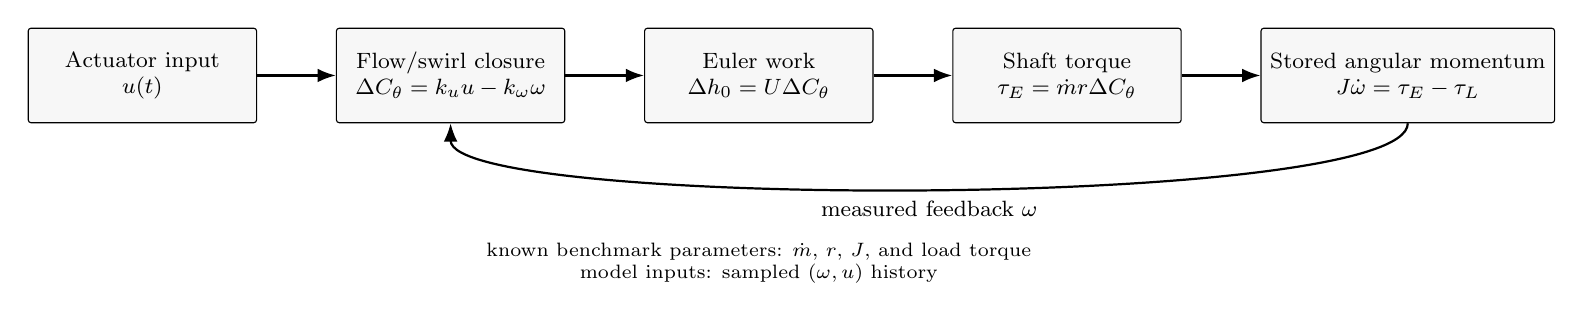
\begin{tikzpicture}[font=\footnotesize, node distance=8mm and 10mm,
  block/.style={draw=black, rounded corners=1pt, fill=gray!6, minimum width=29mm, minimum height=12mm, align=center},
  arrow/.style={-{Latex}, thick, draw=black}]
  \node[block] (control) {Actuator input\\$u(t)$};
  \node[block, right=of control] (flow) {Flow/swirl closure\\$\Delta C_\theta=k_u u-k_\omega\omega$};
  \node[block, right=of flow] (euler) {Euler work\\$\Delta h_0=U\Delta C_\theta$};
  \node[block, right=of euler] (shaft) {Shaft torque\\$\tau_E=\dot m r\Delta C_\theta$};
  \node[block, right=of shaft] (rotor) {Stored angular momentum\\$J\dot\omega=\tau_E-\tau_L$};
  \draw[arrow] (control)--(flow);
  \draw[arrow] (flow)--(euler);
  \draw[arrow] (euler)--(shaft);
  \draw[arrow] (shaft)--(rotor);
  \draw[arrow] (rotor.south) .. controls +(0,-11mm) and +(0,-11mm) .. node[below=1pt]{measured feedback $\omega$} (flow.south);
  \node[below=14mm of euler, align=center, font=\scriptsize] {known benchmark parameters: $\dot m$, $r$, $J$, and load torque\\model inputs: sampled $(\omega,u)$ history};
\end{tikzpicture}
}
 \caption{Reduction from the actuator input to the rotor state. The benchmark makes mass flow, radius, inertia, and load torque explicit, while the learned models receive only sampled speed and control history.}
 \label{fig:physical}
\end{figure*}

\subsection{Linear limit and exact solution}
For $c_2=0$, define
\begin{equation}
 \alpha=\frac{\dot m r k_u}{J},\quad \beta=\frac{\dot m r k_\omega}{J},\quad \gamma=\frac{c_0}{J},\quad
 \omega_\infty=\frac{\alpha u-\gamma}{\beta}.
\end{equation}
For constant control over a step $h$, the exact solution is
\begin{equation}
 \omega(t+h)=\omega_\infty+\left[\omega(t)-\omega_\infty\right]e^{-\beta h},
 \qquad \tau_\mathrm{rotor}=\beta^{-1}.
 \label{eq:exact}
\end{equation}
The corrected short-horizon benchmark uses $k_\omega\in[0.0085,0.0115]$ with a nominal value of $0.01$. Over the stated mass-flow, radius, and inertia ranges, this gives $\beta\approx0.076$--$0.132~\si{\per\second}$, with a nominal value of $0.10~\si{\per\second}$ and a characteristic time of about $10$~s. Its 0.1~s forecast is therefore a short transient, which helps explain why affine identification is such a strong comparator. The separate 2~s nonlinear-load experiment below uses $k_\omega=0.25$ and has a nominal $\beta=2.5~\si{\per\second}$, so it should not be interpreted using the $10$~s time scale.

The nonlinear discrepancy is generated without fabricating a closed-form prediction: $c_2$ is set so that the added load at $400~\si{\radian\per\second}$ is an $\epsilon$ fraction of the total load at that reference speed,
\begin{equation}
 c_2=\frac{\epsilon c_0}{400^2(1-\epsilon)},\qquad \epsilon\in\{0,0.1,0.2,0.5\}.
 \label{eq:c2}
\end{equation}
The exact dynamics are integrated by fourth-order Runge--Kutta with ten internal substeps per $\Delta t=0.01$~s sample. Thus the linear solution in (\ref{eq:exact}) is an analytical verification benchmark, while the nonlinear trajectory is the declared synthetic truth. In the full-trajectory nonlinear-load experiment, $r=0.25~\si{\metre}$, $k_u=8~\si{\metre\per\second}$ per unit control, $k_\omega=0.25~\si{\metre\per\radian}$, and $c_0=0.15~\si{\newton\metre}$; mass flow and inertia are sampled over the ranges reported below.

\subsection{Matrix state-space extension}
The scalar equation is a deliberately reduced version of the control-relevant single-spool structure described by Beneda \emph{et al.}~\cite{beneda2018spool}. A full local linearization uses rotor speed, turbine-inlet pressure, and turbine-inlet temperature perturbations,
\begin{equation}
 \mathbf{x}=\begin{bmatrix}\delta n&\delta p_3^*&\delta T_3^*\end{bmatrix}^{\!T},\qquad
 \dot{\mathbf{x}}=\mathbf{A}\mathbf{x}+\mathbf{B}\delta\dot m_f,\qquad y=\mathbf{C}\mathbf{x},
 \label{eq:ss}
\end{equation}
with $\mathbf{C}=[1\;0\;0]$ for speed measurement. Here $\mathbf{A}$ contains the local derivatives of rotor, combustor mass-storage, and combustor-energy equations; $\mathbf{B}$ contains fuel-flow influence. For constant input over $h$,
\begin{equation}
 \mathbf{x}_{k+1}=\boldsymbol{\Phi}\mathbf{x}_k+\boldsymbol{\Gamma}\mathbf{u}_k,\quad
 \boldsymbol{\Phi}=e^{\mathbf{A}h},\quad
 \boldsymbol{\Gamma}=\int_0^h e^{\mathbf{A}(h-s)}\mathbf{B}\,ds,
 \label{eq:matrix_exact}
\end{equation}
or $\boldsymbol{\Gamma}=\mathbf{A}^{-1}(\boldsymbol{\Phi}-\mathbf{I})\mathbf{B}$ when $\mathbf{A}$ is nonsingular. This full matrix form is a roadmap, not a claim that the present experiment identifies combustor states.

\begin{figure*}[!t]
 \centering
 \resizebox{0.96\textwidth}{!}{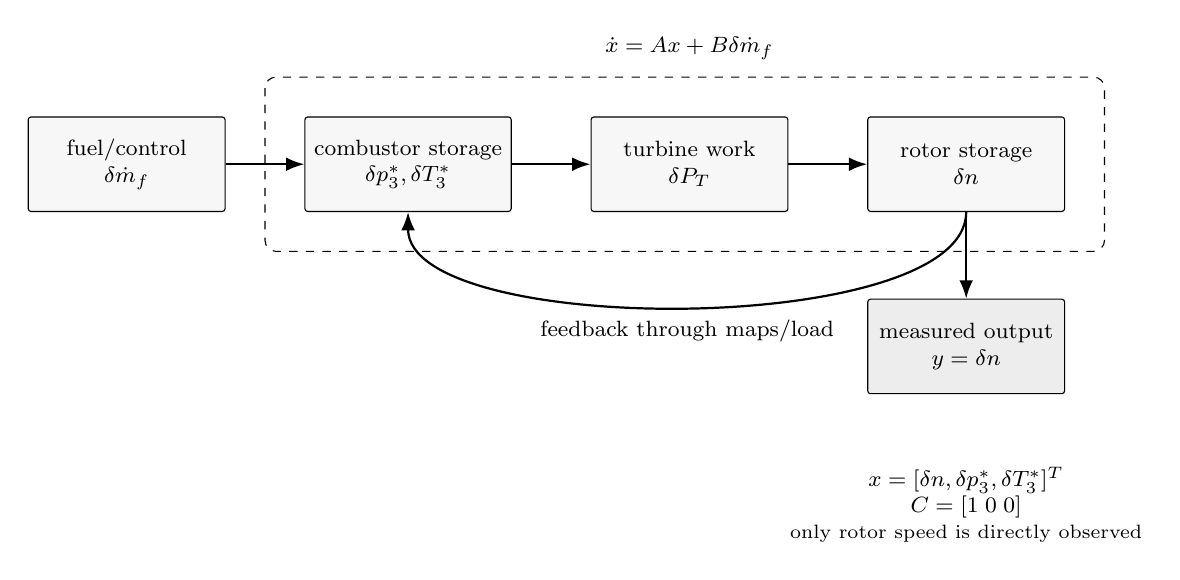
\begin{tikzpicture}[font=\footnotesize, node distance=8mm and 10mm,
  state/.style={draw=black, rounded corners=1pt, fill=gray!6, minimum width=25mm, minimum height=12mm, align=center},
  arrow/.style={-{Latex}, thick, draw=black}]
  \node[state] (fuel) {fuel/control\\$\delta\dot m_f$};
  \node[state, right=of fuel] (comb) {combustor storage\\$\delta p_3^*,\delta T_3^*$};
  \node[state, right=of comb] (turb) {turbine work\\$\delta P_T$};
  \node[state, right=of turb] (rotor) {rotor storage\\$\delta n$};
  \node[state, fill=gray!14, below=11mm of rotor] (out) {measured output\\$y=\delta n$};
  \draw[arrow] (fuel)--(comb);
  \draw[arrow] (comb)--(turb);
  \draw[arrow] (turb)--(rotor);
  \draw[arrow] (rotor)--(out);
  \draw[arrow] (rotor.south) .. controls +(0,-16mm) and +(0,-16mm) .. node[below=1pt]{feedback through maps/load} (comb.south);
  \draw[draw=black, dashed, rounded corners] ([xshift=-5mm,yshift=5mm]comb.north west) rectangle ([xshift=5mm,yshift=-5mm]rotor.south east);
  \node[above=6mm of turb, align=center] {$\dot{x}=Ax+B\delta\dot m_f$};
  \node[below=8mm of out, align=center] {$x=[\delta n,\delta p_3^*,\delta T_3^*]^T$\\$C=[1\;0\;0]$\\\scriptsize only rotor speed is directly observed};
\end{tikzpicture}
}
 \caption{State-space scaffold for the next model scale. The present study keeps only the rotor state; combustor pressure and temperature are shown as future states, not identified variables.}
 \label{fig:matrix}
\end{figure*}

\section{Causal learning framework}
The two neural models serve different purposes. The gated recurrent unit (GRU) is the easier one to interpret: it is a recurrent neural network with a learned memory. It reads the context one sample at a time and uses gates to decide what information from the recent history to retain. Here, the GRU is a direct supervised comparator. It receives the context and is trained against the future trajectory, so its main loss is measured in the same physical quantity that we ultimately care about: rotor-speed error.

The GRU is a small learned memory, not another physical law. At each sample, it combines the current input with its previous hidden state. An update gate decides how much of the old memory to keep, while a reset gate controls how much of the old memory enters the new candidate state. In a standard GRU notation,
\begin{equation}
 \begin{aligned}
 r_t&=\sigma(W_r x_t+U_r h_{t-1}),\\
 z_t&=\sigma(W_z x_t+U_z h_{t-1}),\\
 \tilde h_t&=\tanh(W_hx_t+U_h(r_t\odot h_{t-1})),\\
 h_t&=(1-z_t)\odot h_{t-1}+z_t\odot\tilde h_t.
 \end{aligned}
\end{equation}
The gates and weights are learned from the training sequences; they are not estimates of inertia, torque, or any other physical coefficient. In this experiment, the GRU reads the same 20-step context of sampled rotor speed and control as the hybrid model, compresses that history into its hidden state, and uses a supervised output head to predict the future rotor trajectory.

The joint-embedding predictive architecture (JEPA) takes a different route. During training, one encoder reads the observed context and a second, stop-gradient encoder reads the future target. A predictor is trained to make the context representation match the future representation. The target encoder is updated by an exponential moving average (EMA), rather than by backpropagation. At inference, the future branch is removed. The model sees only the context and known control, then adds a learned correction to the calibrated physics forecast. The GRU is therefore a direct sequence predictor, while JEPA is a representation-prediction objective attached to a physics-based forecast. A lower latent loss does not by itself show that the decoded rotor trajectory is more accurate or more physically consistent.

The comparison is controlled at the information boundary. Both models receive the same observed context and control, and both are evaluated on the same held-out 200-step future. The difference is the learning question: the GRU asks whether a sequence model can directly reduce rotor-speed error, whereas JEPA asks whether predicting a future latent representation is a useful way to learn a residual on top of the calibrated rotor equation. The evaluation then checks more than the training objective: trajectory RMSE, ODE residual, forecast-horizon error, and finite-difference control sensitivity. This separation prevents a representation score from being mistaken for an engineering result.

For the full-trajectory nonlinear-load experiment, each example contains a 20-step context $x_{0:19}=[\omega_t/600,u_t]$ and a 200-step future target $y_{20:219}$ under a known constant control. Training sequences use $\dot m\in[0.70,0.90]~\si{\kilogram\per\second}$, $J\in[0.017,0.023]~\si{\kilogram\metre\squared}$, $u\in[0.45,1.05]$, and $\omega_0\in[350,450]~\si{\radian\per\second}$. There are 120 training and 30 test sequences per $\epsilon$; 20\% of training sequences are held out for checkpoint selection. The test set is never used for tuning. This is the experiment behind Table~\ref{tab:rmse} and the nonlinear diagnostic figures. Figure~\ref{fig:analytical} instead comes from the separate corrected short-horizon benchmark, which uses a 10-step, 0.1~s forecast and the source parameter range $k_\omega\in[0.0085,0.0115]$.

The context encoder is a GRU with 48 hidden units, followed by $48\rightarrow24\rightarrow24$ projection. The target encoder has the same structure. The predictor receives the 24-dimensional context embedding and the final control, and the trajectory head receives the same 25 features and returns all 200 residual samples. The forecast is
\begin{equation}
  \begin{aligned}
  \hat{\boldsymbol\omega}&=\boldsymbol\omega^{\,\mathrm{cal}}+600h(z_c,u),\\
  z_c&=E_c(x_{0:19}),\qquad z_y=\operatorname{sg}(E_y(y_{20:219})).
  \end{aligned}
 \label{eq:architecture}
\end{equation}
where $\boldsymbol\omega^{\,\mathrm{cal}}$ is a local affine rollout fit from the context and $\operatorname{sg}$ denotes stop-gradient. The objective combines a trajectory mean-squared error (MSE) term with a latent matching term. The target representation is first passed through layer normalization (LN):
\begin{equation}
  \begin{aligned}
  \mathcal{L}={}&\operatorname{MSE}\!\left(h(z_c,u),
  \frac{\boldsymbol\omega-\boldsymbol\omega^{\,\mathrm{cal}}}{600}\right)\\
  &+0.05\left\|P(z_c,u)-\operatorname{LN}(z_y)\right\|_1.
  \end{aligned}
 \label{eq:loss}
\end{equation}
The target encoder is not available at inference and is updated only by EMA,
\begin{equation}
  \begin{aligned}
  \theta_y&\leftarrow m\theta_y+(1-m)\theta_c,\\
  m&=1-(1-0.998)\frac{1+\cos(\pi s/1000)}{2}.
  \end{aligned}
 \label{eq:ema}
\end{equation}
where $s$ is the gradient step. This is a scalar, GRU-based translation of the target-normalization, stop-gradient, and EMA ideas in JEPA literature; it is not an image/video JEPA reproduction~\cite{assran2023ijepa,bardes2024vjepa,assran2025vjepa2}.

\begin{figure*}[!t]
 \centering
 \resizebox{0.96\textwidth}{!}{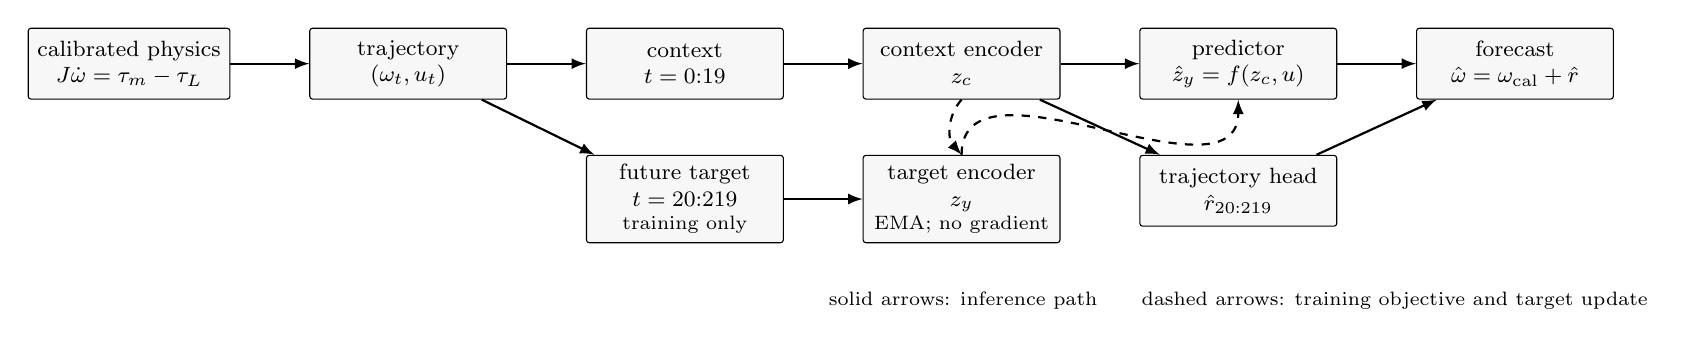
\begin{tikzpicture}[font=\footnotesize, node distance=7mm and 10mm,
  box/.style={draw=black, rounded corners=1pt, fill=gray!6, align=center, minimum height=9mm, minimum width=25mm},
  arrow/.style={-latex, thick, draw=black}, dashedarrow/.style={-latex, thick, dashed, draw=black}]
\node[box] (physics) {calibrated physics\\$J\dot\omega=\tau_m-\tau_L$};
\node[box, right=of physics] (data) {trajectory\\$(\omega_t,u_t)$};
\node[box, right=of data] (split) {context\\$t=0{:}19$};
\node[box, below=of split] (future) {future target\\$t=20{:}219$\\[-1pt]{\scriptsize training only}};
\node[box, right=of split] (encoder) {context encoder\\$z_c$};
\node[box, right=of future] (target) {target encoder\\$z_y$\\[-1pt]{\scriptsize EMA; no gradient}};
\node[box, right=of encoder] (predictor) {predictor\\$\hat z_y=f(z_c,u)$};
\node[box, below=of predictor] (head) {trajectory head\\$\hat r_{20:219}$};
\node[box, right=of predictor] (output) {forecast\\$\hat\omega=\omega_{\rm cal}+\hat r$};
\draw[arrow] (physics)--(data); \draw[arrow] (data)--(split); \draw[arrow] (data)--(future);
\draw[arrow] (split)--(encoder); \draw[arrow] (future)--(target); \draw[arrow] (encoder)--(predictor);
\draw[arrow] (predictor)--(output); \draw[arrow] (encoder)--(head); \draw[arrow] (head)--(output);
\draw[dashedarrow] (target.north) to[out=90,in=-90] (predictor.south);
\draw[dashedarrow] (encoder.south) to[bend right=42] (target.north);
\node[below=7mm of head, align=center, font=\scriptsize] {solid arrows: inference path\qquad dashed arrows: training objective and target update};
\end{tikzpicture}
}
 \caption{Training and inference paths for the JEPA-style hybrid. The future trajectory enters only the stop-gradient target branch during training. At inference, the model uses the context and known control to add a learned residual to calibrated physics.}
 \label{fig:jepa}
\end{figure*}

\begin{figure*}[!t]
 \centering
 \resizebox{0.96\textwidth}{!}{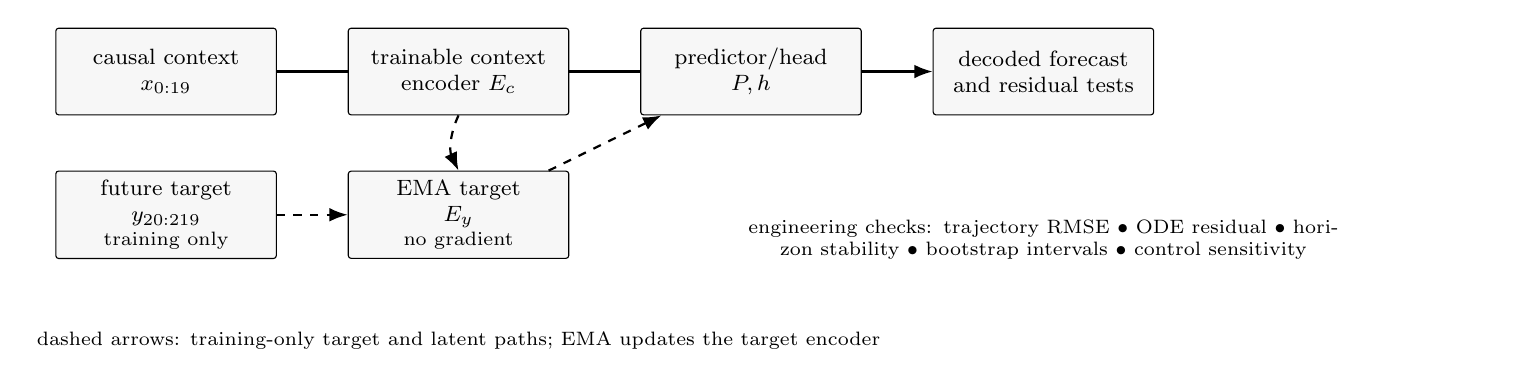
\begin{tikzpicture}[font=\footnotesize, node distance=7mm and 9mm,
  box/.style={draw=black, rounded corners=1pt, fill=gray!6, minimum width=28mm, minimum height=11mm, align=center},
  arrow/.style={-{Latex}, thick, draw=black}, dashedarrow/.style={-{Latex}, thick, dashed, draw=black}]
  \node[box] (context) {causal context\\$x_{0:19}$};
  \node[box, right=of context] (enc) {trainable context\\encoder $E_c$};
  \node[box, right=of enc] (pred) {predictor/head\\$P,h$};
  \node[box, right=of pred] (diag) {decoded forecast\\and residual tests};
  \node[box, below=of context] (future) {future target\\$y_{20:219}$\\[-1pt]{\scriptsize training only}};
  \node[box, right=of future] (target) {EMA target\\$E_y$\\[-1pt]{\scriptsize no gradient}};
  \draw[arrow] (context)--(enc)--(pred)--(diag);
  \draw[dashedarrow] (future)--(target);
  \draw[dashedarrow] (target)--(pred);
  \draw[dashedarrow] (enc.south) to[bend right=25] (target.north);
  \node[below=8mm of target, align=left, font=\scriptsize] {dashed arrows: training-only target and latent paths; EMA updates the target encoder};
  \node[below=12mm of diag, align=center, text width=112mm, font=\scriptsize] {engineering checks: trajectory RMSE $\bullet$ ODE residual $\bullet$ horizon stability $\bullet$ bootstrap intervals $\bullet$ control sensitivity};
\end{tikzpicture}
}
 \caption{Checks that keep the latent objective tied to engineering quantities. The forecast is decoded and then evaluated using trajectory error, ODE residual, horizon stability, bootstrap intervals, and control sensitivity.}
 \label{fig:transparency}
\end{figure*}

\section{Evaluation and verification}
The supervised baseline is a GRU residual model with the same 48-unit encoder scale and a $48\rightarrow96\rightarrow200$ trajectory head. Other baselines are persistence, two-point extrapolation, raw-context ordinary least squares (OLS), least-squares transition identification, nominal physics, calibrated physics, and a true-parameter integration oracle. The baseline suite establishes that the corrected linear benchmark is nearly affine; it is not a weak comparator selection.

For $N$ sequences and horizon $H$, we report
\begin{equation}
  \begin{aligned}
  \mathrm{RMSE}_{\mathrm{traj}}&=\sqrt{\frac{1}{NH}\sum_{i=1}^{N}\sum_{j=1}^{H}
  (\hat\omega_{ij}-\omega_{ij})^2},\\
  e_\tau&=J\frac{\hat\omega_{j+1}-\hat\omega_j}{\Delta t}
  -\tau_{\mathrm{rhs}}(\hat\omega_j,u_j),\\
  \tau_{\mathrm{rhs}}(\omega,u)&=\dot m r(k_u u-k_\omega\omega)-c_0-c_2\omega^2.
  \end{aligned}
\end{equation}
We also report endpoint RMSE, $R^2$, skill versus persistence, horizon error at 0.1--2.0~s, and sequence-level bootstrap intervals. Control sensitivity is a finite-difference endpoint derivative diagnostic: the reported value is the RMSE between the model derivative and a fresh exact-dynamics derivative after a $\Delta u=10^{-3}$ perturbation. It is not controller validation.

\begin{figure*}[!t]
 \centering
 \resizebox{0.96\textwidth}{!}{\begin{tikzpicture}
\begin{groupplot}[group style={group size=2 by 1, horizontal sep=1.55cm}, width=0.44\textwidth, height=0.25\textwidth, xlabel={gradient step}, tick align=inside, grid=none, minor tick num=1]
\nextgroupplot[ymode=log, ylabel={training objective}, legend style={font=\scriptsize, draw=none, at={(0.5,1.13)}, anchor=south, legend columns=2, /tikz/every even column/.append style={column sep=4pt}}]
  \addplot[black, thick, mark=none] table[x=gradient_step,y=train_loss,col sep=comma] {../reports/paper_history_gru_residual_7_eps05.csv};
  \addlegendentry{GRU, seed 7}
  \addplot[black, dashed, thick, mark=none] table[x=gradient_step,y=train_loss,col sep=comma] {../reports/paper_history_jepa_residual_7_eps05.csv};
  \addlegendentry{JEPA, seed 7}
\nextgroupplot[ylabel={validation RMSE (\si{\radian\per\second})}, legend style={font=\scriptsize, draw=none, at={(0.5,1.13)}, anchor=south, legend columns=2, /tikz/every even column/.append style={column sep=3pt}}]
  \addplot[black, thick, mark=none] table[x=gradient_step,y=validation_trajectory_rmse_rad_s,col sep=comma] {../reports/paper_history_gru_residual_7_eps05.csv};
  \addplot[black, dashed, mark=none] table[x=gradient_step,y=validation_trajectory_rmse_rad_s,col sep=comma] {../reports/paper_history_gru_residual_19_eps05.csv};
  \addplot[black, dotted, mark=none] table[x=gradient_step,y=validation_trajectory_rmse_rad_s,col sep=comma] {../reports/paper_history_gru_residual_31_eps05.csv};
  \addlegendentry{GRU: solid/dashed/dotted = 7/19/31}
  \addplot[black!55, thick, mark=none] table[x=gradient_step,y=validation_trajectory_rmse_rad_s,col sep=comma] {../reports/paper_history_jepa_residual_7_eps05.csv};
  \addplot[black!55, dashed, mark=none] table[x=gradient_step,y=validation_trajectory_rmse_rad_s,col sep=comma] {../reports/paper_history_jepa_residual_19_eps05.csv};
  \addplot[black!55, dotted, mark=none] table[x=gradient_step,y=validation_trajectory_rmse_rad_s,col sep=comma] {../reports/paper_history_jepa_residual_31_eps05.csv};
  \addlegendentry{JEPA: solid/dashed/dotted = 7/19/31}
\end{groupplot}
\end{tikzpicture}
}
 \caption{Training objective and held-out trajectory error at $\epsilon=0.5$. The GRU improves steadily over the displayed budget; JEPA is more variable across seeds, and lower latent loss does not translate into lower physical error.}
 \label{fig:training}
\end{figure*}

\section{Results}
\subsection{Analytical benchmark and nonlinear discrepancy}
The corrected linear benchmark shows why the original endpoint claim was uninformative: persistence has RMSE $1.6063$, two-point extrapolation $0.0092$, raw-context OLS $6.8\times10^{-5}$, nominal analytical physics $0.4607$, and least-squares system identification $6.8\times10^{-5}$~\si{\radian\per\second}. The original JEPA context probe was approximately $26.4$~\si{\radian\per\second}; the short horizon and nearly affine dynamics make ordinary identification a decisive baseline.

\begin{figure}[!t]
 \centering
 \pgfplotsset{compat=1.18}
\begin{tikzpicture}
\begin{axis}[
  width=\columnwidth,
  height=0.92\columnwidth,
  xlabel={True $\omega$ (\si{\radian\per\second})},
  ylabel={Predicted $\omega$ (\si{\radian\per\second})},
  legend style={draw=none, font=\scriptsize, at={(0.5,1.10)}, anchor=south, legend columns=2, /tikz/every even column/.append style={column sep=4pt}},
  xmin=340, xmax=530,
  ymin=340, ymax=530,
  axis equal image,
  tick align=inside,
  minor tick num=1,
  grid=none,
]
  \addplot[black!55, dashed, no marks, domain=340:530] {x};
  \addlegendentry{exact prediction}
  % Numeric values are read from the reproducible CSV output.
  \addplot+[only marks, mark=o, mark size=1.1pt, black]
    table [x=true_omega_rad_s, y=jepa_probe_omega_rad_s, col sep=comma]
    {../results/corrected_predictions.csv};
  \addlegendentry{JEPA + probe}
  \addplot+[only marks, mark=square, mark size=1.1pt, black]
    table [x=true_omega_rad_s, y=nominal_analytical_omega_rad_s, col sep=comma]
    {../results/corrected_predictions.csv};
  \addlegendentry{Nominal analytical}
  \addplot+[only marks, mark=diamond*, black]
    table [x=true_omega_rad_s, y=oracle_analytical_omega_rad_s, col sep=comma]
    {../results/corrected_predictions.csv};
  \addlegendentry{True-parameter oracle}
\end{axis}
\end{tikzpicture}

 \caption{Endpoint predictions for the corrected linear benchmark. The diagonal represents exact prediction. The true-parameter oracle follows it, while the JEPA probe remains close to the observed-speed band.}
 \label{fig:analytical}
\end{figure}

\begin{table}[!t]
\caption{Mean held-out full-trajectory RMSE in \si{\radian\per\second}.}
\label{tab:rmse}
\centering\scriptsize
\begin{tabular}{lrrrr}
\toprule
Method & $\epsilon=0$ & .1 & .2 & .5\\
\midrule
Nominal physics & 5.392 & 5.388 & 5.384 & 5.362\\
Calibrated physics & $\,.0003$ & .130 & .293 & 1.160\\
Supervised GRU & .057 & .059 & .065 & .125\\
JEPA-style hybrid & .441 & .423 & .393 & .493\\
\bottomrule
\end{tabular}
\end{table}

The nonlinear-load sweep, forecast-horizon comparison, and control-sensitivity diagnostic are collected in Appendix~\ref{app:diagnostics} so that the main results and references remain easier to read.

At $\epsilon=0.5$, full-trajectory JEPA is indeed lower than calibrated physics ($0.4933$ versus $1.1603$~\si{\radian\per\second}), correcting the earlier claim. It remains about 4.0 times worse than the GRU ($0.1248$), and its mean ODE residual is approximately $1.24$~\si{\newton\metre} across seeds versus $0.168$~\si{\newton\metre} for the GRU and $0.096$~\si{\newton\metre} for calibrated physics. Thus the latent objective improves neither the strongest learned trajectory metric nor physical consistency.

\subsection{Optimization, reachability, and control sensitivity}
The GRU selected 975--1000 gradient steps for all conditions, so the stated budget remains a ceiling. JEPA selected 200--1000 steps depending on load and seed, which is evidence of optimization sensitivity rather than a stable optimum. The earlier representation audit also found that variance/covariance regularization improved endpoint-probe RMSE from about $26.42$ to $25.47$~\si{\radian\per\second}, but effective rank remained near $1$ of $24$ dimensions. A lower latent loss therefore cannot be treated as a richer or more physical state representation.

The reachability check found a 430~\si{\radian\per\second} target infeasible under the selected control bounds: the reachable terminal set was $[395.49,414.31]$~\si{\radian\per\second}. The remaining gap must be established before reward shaping, model-predictive control (MPC), or reinforcement learning; optimizing an unreachable target would confound objective and actuator limitations.

The corrected second sensitivity audit gives a different failure mode. Nominal physics has sensitivity error $0.114$--$0.122$~\si{\radian\per\second} per unit control across the sweep, while calibrated physics is about $31.75$--$31.79$ and the learned residual models are about $31.38$--$32.02$ in the same diagnostic. The latter models are therefore nearly control-insensitive under the present experiment. This is a limitation of the calibration and model-input design: a single constant-control context and a residual head do not force the learned correction to preserve control derivatives. It is not a general JEPA conclusion.

\section{Discussion, limitations, and work in progress}
The result is consistent with the physics of this benchmark. Calibrated physics receives a context-derived local transition, so it is nearly exact over the short forecast. The supervised GRU receives the same residual target directly and learns the quantity that is scored. The JEPA-style model adds a summary embedding and a latent target, but its direct forecast head is not required to preserve per-step control authority or the governing differential equation. The present failure is therefore a mismatch between the representation objective and the engineering tests. It is not evidence that feature prediction is intrinsically unsuitable.

The next model should grow in a physically specific direction. Compressor work and flow maps would drive combustor pressure and energy storage. Combustion delay and heat release would drive turbine-inlet temperature. Turbine work would then close the rotor balance. The three-state matrix structure in (\ref{eq:ss}) provides a starting scaffold, while published micro-turbojet studies show why linear local models and nonlinear system identification need to be compared across operating zones~\cite{beneda2018spool,shehata2024microturbojet}. The present study does not connect UIUC section polars to the transient rotor model; that aerodynamic-to-rotor coupling remains future work.

\subsection{Work in progress}
This project is ongoing, and the present paper is an intermediate method-development result rather than a finished engine model. The immediate improvements are to use per-step action-conditioned target tokens, causally unroll the latent state, vary the control during the forecast, include delayed actuation and parameter drift, and test on held-out dynamical regimes. The evaluation will continue to require decoded trajectory error, ODE residuals, horizon stability, and control sensitivity. After that, the benchmark should be connected to experimentally anchored compressor--combustor--turbine data with explicit state estimation and uncertainty reporting. These steps are still in progress; they are the work needed before the method can support claims about a real propulsion system.

\section{Conclusions and claim boundary}
The corrected experiment answers the stated question negatively for this implementation. At $\epsilon=0.5$, the JEPA-style hybrid is better than calibrated physics in full-trajectory RMSE, but it remains worse than the supervised GRU and has substantially larger ODE residuals. The control audit further shows that the calibrated and learned residual models lose endpoint control sensitivity under the current input design, whereas nominal physics preserves it. These are useful failure modes because they point to specific changes in the model and experiment.

The study is synthetic, scalar, and prediction-only. It has no experimental validation, no real compressor or combustor maps, and no controller deployment. The supported conclusion is therefore methodological: a JEPA-style dynamics learner can be audited transparently, but this implementation is not yet a validated world model. Improvements remain in progress, especially the move to a multi-state, action-conditioned, experimentally anchored compressor--combustor--turbine model with explicit state estimation, uncertainty reporting, and regime-held-out validation.

\bibliographystyle{IEEEtran}
\bibliography{references}
\clearpage
\onecolumn
\appendices
\section{Additional diagnostic figures}\label{app:diagnostics}
The figures in this appendix contain the remaining diagnostics from the corrected nonlinear-load experiment. They are included for completeness, but they do not change the claim boundary in the main text.

\begin{center}
\refstepcounter{figure}\label{fig:summary}
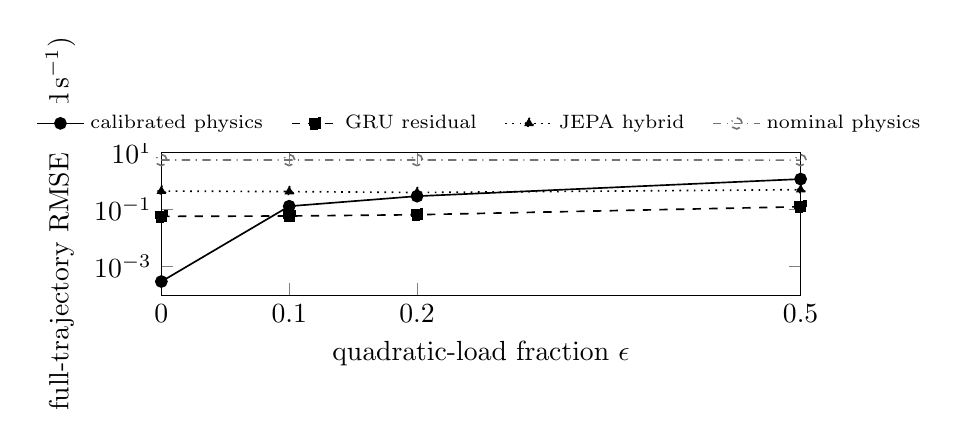
\begin{tikzpicture}
\begin{axis}[width=0.80\textwidth,height=0.28\textwidth,xlabel={quadratic-load fraction $\epsilon$},ylabel={full-trajectory RMSE (\si{\radian\per\second})},xmin=0,xmax=.5,ymin=1e-4,ymax=10,ymode=log,grid=none,minor y tick num=1,legend style={font=\scriptsize,draw=none,at={(0.5,1.06)},anchor=south,legend columns=4,/tikz/every even column/.append style={column sep=0.8em}},xtick={0,.1,.2,.5}]
\addplot[black,solid,semithick,mark=*] coordinates {(0,.0003) (.1,.1302) (.2,.2925) (.5,1.1603)};\addlegendentry{calibrated physics}
\addplot[black,dashed,semithick,mark=square*] coordinates {(0,.0573) (.1,.0591) (.2,.0655) (.5,.1248)};\addlegendentry{GRU residual}
\addplot[black,dotted,semithick,mark=triangle*] coordinates {(0,.4412) (.1,.4227) (.2,.3933) (.5,.4933)};\addlegendentry{JEPA hybrid}
\addplot[black!55,dashdotted,semithick,mark=o] coordinates {(0,5.3921) (.1,5.3884) (.2,5.3839) (.5,5.3620)};\addlegendentry{nominal physics}
\end{axis}
\end{tikzpicture}

\par\smallskip
\parbox{0.80\textwidth}{\textbf{Fig.~\thefigure.} Held-out full-trajectory root-mean-square error as the quadratic-load fraction increases. At $\epsilon=0.5$, the JEPA-style hybrid is better than calibrated physics but remains worse than the supervised gated recurrent unit.}

\par\medskip
\refstepcounter{figure}\label{fig:horizon}
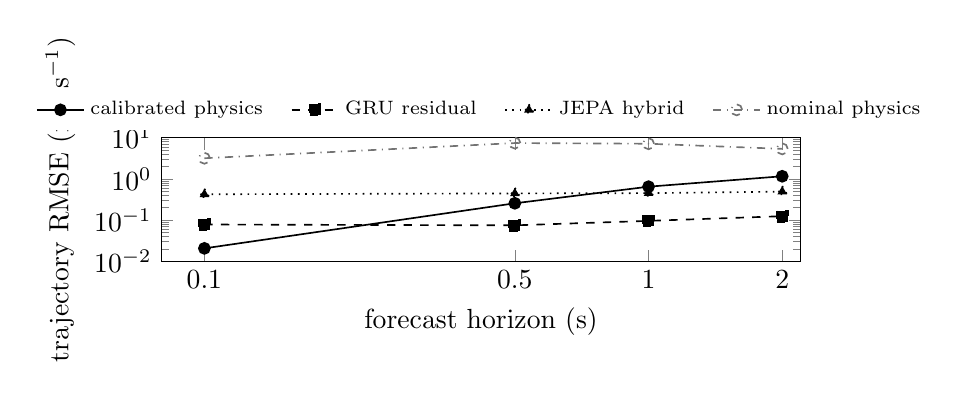
\begin{tikzpicture}
\begin{axis}[width=0.80\textwidth,height=0.26\textwidth, xmode=log, ymode=log, xlabel={forecast horizon (s)}, ylabel={trajectory RMSE (\si{\radian\per\second})}, xmin=.08,xmax=2.2,ymin=.01,ymax=10, xtick={.1,.5,1,2}, xticklabels={$0.1$,$0.5$,$1$,$2$}, grid=none, minor tick num=1, legend style={font=\scriptsize, draw=none, at={(0.5,1.06)}, anchor=south, legend columns=4,/tikz/every even column/.append style={column sep=0.8em}}]
  \addplot[black, solid, semithick, mark=*] coordinates {(.1,.0207) (.5,.2566) (1,.6487) (2,1.1603)}; \addlegendentry{calibrated physics}
  \addplot[black, dashed, semithick, mark=square*] coordinates {(.1,.0784) (.5,.0749) (1,.0961) (2,.1248)}; \addlegendentry{GRU residual}
  \addplot[black, dotted, semithick, mark=triangle*] coordinates {(.1,.4244) (.5,.4455) (1,.4523) (2,.4933)}; \addlegendentry{JEPA hybrid}
  \addplot[black!55, dashdotted, semithick, mark=o] coordinates {(.1,3.177) (.5,7.409) (1,7.142) (2,5.362)}; \addlegendentry{nominal physics}
\end{axis}
\end{tikzpicture}

\par\smallskip
\parbox{0.80\textwidth}{\textbf{Fig.~\thefigure.} Held-out trajectory error versus forecast horizon at $\epsilon=0.5$. Calibrated physics accumulates discrepancy, while the gated recurrent unit remains the most accurate over the tested horizon.}

\par\medskip
\refstepcounter{figure}\label{fig:sensitivity}
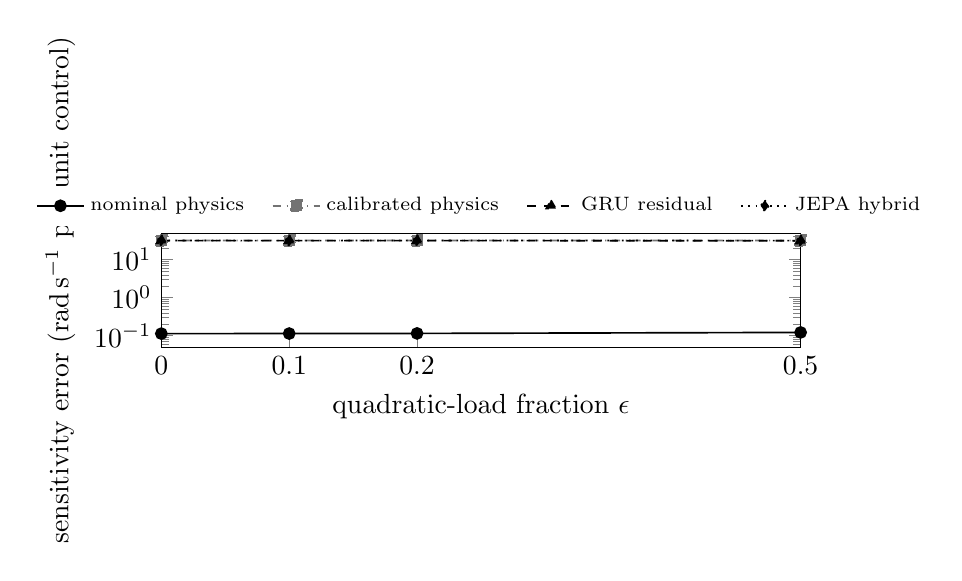
\begin{tikzpicture}
\begin{axis}[width=0.80\textwidth,height=0.25\textwidth, xlabel={quadratic-load fraction $\epsilon$}, ylabel={sensitivity error (\si{\radian\per\second} per unit control)}, xmin=0,xmax=.5,ymin=.05,ymax=50,ymode=log, xtick={0,.1,.2,.5}, grid=none, minor y tick num=1, legend style={font=\scriptsize, draw=none, at={(0.5,1.06)}, anchor=south, legend columns=4,/tikz/every even column/.append style={column sep=0.8em}}]
  \addplot[black, solid, semithick, mark=*] coordinates {(0,.1138) (.1,.1143) (.2,.1152) (.5,.1223)}; \addlegendentry{nominal physics}
  \addplot[black!55, dashdotted, semithick, mark=square*] coordinates {(0,31.7855) (.1,31.7815) (.2,31.7772) (.5,31.7523)}; \addlegendentry{calibrated physics}
  \addplot[black, dashed, semithick, mark=triangle*] coordinates {(0,31.7166) (.1,31.6814) (.2,31.6369) (.5,31.3821)}; \addlegendentry{GRU residual}
  \addplot[black, dotted, semithick, mark=diamond*] coordinates {(0,32.0246) (.1,31.5194) (.2,32.0010) (.5,31.6104)}; \addlegendentry{JEPA hybrid}
\end{axis}
\end{tikzpicture}

\par\smallskip
\parbox{0.80\textwidth}{\textbf{Fig.~\thefigure.} Error in the finite-difference control sensitivity. Nominal physics preserves the exact sensitivity, whereas the calibrated and learned residual models lose it under the constant-control protocol.}
\end{center}

\section{Matrix algebra and residual decomposition}\label{app:matrix}
The scalar benchmark is useful because every term can be checked by hand. The next model scale needs the same discipline, but with several coupled states. This appendix writes out that extension and shows where the present residual model sits inside it. The matrix equations are a modelling scaffold; the current experiment does not identify the pressure or temperature states.

\subsection{Nonlinear state equations and local linearization}
Let the physical state be
\begin{equation}
  \mathbf{x}=\begin{bmatrix}\omega & p_3 & T_3\end{bmatrix}^{T},
  \qquad
  \dot{\mathbf{x}}=\mathbf{f}(\mathbf{x},\mathbf{u};\boldsymbol{\theta}),
  \qquad
  \mathbf{y}=\mathbf{g}(\mathbf{x},\mathbf{u}),
  \label{eq:app_nonlinear_state}
\end{equation}
where $\omega$ is rotor speed, $p_3$ is a combustor or turbine-inlet pressure state, $T_3$ is a turbine-inlet temperature state, and $\mathbf{u}$ collects commanded fuel flow and any other measured actuators. The parameter vector $\boldsymbol{\theta}$ contains inertia, volumes, map coefficients, heat capacities, and loss parameters. A steady operating point $(\bar{\mathbf{x}},\bar{\mathbf{u}})$ satisfies $\mathbf{f}(\bar{\mathbf{x}},\bar{\mathbf{u}};\boldsymbol{\theta})=\mathbf{0}$. Define perturbations
\begin{equation}
  \delta\mathbf{x}=\mathbf{x}-\bar{\mathbf{x}},
  \qquad
  \delta\mathbf{u}=\mathbf{u}-\bar{\mathbf{u}},
  \qquad
  \delta\mathbf{y}=\mathbf{y}-\bar{\mathbf{y}}.
\end{equation}
The first-order Taylor expansion is
\begin{equation}
  \delta\dot{\mathbf{x}}
  =\underbrace{\left.\frac{\partial\mathbf{f}}{\partial\mathbf{x}}\right|_{\bar{\mathbf{x}},\bar{\mathbf{u}}}}_{\mathbf{A}}
   \delta\mathbf{x}
  +\underbrace{\left.\frac{\partial\mathbf{f}}{\partial\mathbf{u}}\right|_{\bar{\mathbf{x}},\bar{\mathbf{u}}}}_{\mathbf{B}}
   \delta\mathbf{u}
  +\mathcal{O}\!\left(\|\delta\mathbf{x},\delta\mathbf{u}\|^2\right),
  \qquad
  \delta\mathbf{y}=\mathbf{C}\delta\mathbf{x}+\mathbf{D}\delta\mathbf{u},
  \label{eq:app_linearization}
\end{equation}
with $\mathbf{C}=\partial\mathbf{g}/\partial\mathbf{x}$ and $\mathbf{D}=\partial\mathbf{g}/\partial\mathbf{u}$ evaluated at the same operating point. The matrices are local derivatives, not universal engine constants. They change with operating condition.

For the scalar rotor equation used in the paper,
\begin{equation}
  J\dot{\omega}=\dot m r(k_u u-k_\omega\omega)-c_0-c_2\omega^2,
\end{equation}
the local derivatives are explicit:
\begin{equation}
  A_\omega=-\frac{\dot m r k_\omega+2c_2\bar\omega}{J},
  \qquad
  B_u=\frac{\dot m r k_u}{J}.
  \label{eq:app_scalar_jacobian}
\end{equation}
This makes the physical meaning of the matrix entries concrete. $A_\omega$ is the local speed feedback, including the slope of the quadratic load, and $B_u$ is the local control authority.

\subsection{Exact zero-order-hold discretization}
Assume the input is constant over one sample interval $h$. The solution of the linearized system is
\begin{equation}
  \delta\mathbf{x}(t+h)
  =e^{\mathbf{A}h}\delta\mathbf{x}(t)
  +\int_0^h e^{\mathbf{A}(h-s)}\mathbf{B}\,\delta\mathbf{u}(t)\,\mathrm{d}s.
\end{equation}
Define
\begin{equation}
  \boldsymbol{\Phi}=e^{\mathbf{A}h},
  \qquad
  \boldsymbol{\Gamma}=\int_0^h e^{\mathbf{A}(h-s)}\mathbf{B}\,\mathrm{d}s.
\end{equation}
Then the exact zero-order-hold update is
\begin{equation}
  \delta\mathbf{x}_{k+1}=\boldsymbol{\Phi}\delta\mathbf{x}_k
  +\boldsymbol{\Gamma}\delta\mathbf{u}_k,
  \qquad
  \delta\mathbf{y}_k=\mathbf{C}\delta\mathbf{x}_k+\mathbf{D}\delta\mathbf{u}_k.
  \label{eq:app_zoh}
\end{equation}
When $\mathbf{A}$ is nonsingular, the input matrix can also be written as
\begin{equation}
  \boldsymbol{\Gamma}=\mathbf{A}^{-1}(\boldsymbol{\Phi}-\mathbf{I})\mathbf{B}.
  \label{eq:app_gamma_inverse}
\end{equation}
The inverse formula is convenient on paper but is not the safest numerical implementation when $\mathbf{A}$ is ill-conditioned. A block matrix exponential avoids explicitly forming $\mathbf{A}^{-1}$:
\begin{equation}
  \exp\!\left(
  h\begin{bmatrix}\mathbf{A}&\mathbf{B}\\\mathbf{0}&\mathbf{0}\end{bmatrix}\right)
  =\begin{bmatrix}\boldsymbol{\Phi}&\boldsymbol{\Gamma}\\\mathbf{0}&\mathbf{I}\end{bmatrix}.
  \label{eq:app_block_exponential}
\end{equation}

After $N$ steps, the state is
\begin{equation}
  \delta\mathbf{x}_{k+N}
  =\boldsymbol{\Phi}^{N}\delta\mathbf{x}_k
  +\sum_{j=0}^{N-1}\boldsymbol{\Phi}^{N-1-j}\boldsymbol{\Gamma}\delta\mathbf{u}_{k+j}.
  \label{eq:app_multistep}
\end{equation}
For a constant perturbation $\delta\mathbf{u}$, the endpoint control derivative is therefore
\begin{equation}
  \frac{\partial\delta\mathbf{x}_{k+N}}{\partial\delta\mathbf{u}}
  =\left(\sum_{j=0}^{N-1}\boldsymbol{\Phi}^{j}\right)\boldsymbol{\Gamma},
  \qquad
  \frac{\partial\delta\mathbf{y}_{k+N}}{\partial\delta\mathbf{u}}
  =\mathbf{C}\left(\sum_{j=0}^{N-1}\boldsymbol{\Phi}^{j}\right)\boldsymbol{\Gamma}+\mathbf{D}.
  \label{eq:app_sensitivity}
\end{equation}
Equation~(\ref{eq:app_sensitivity}) is the matrix version of the finite-difference control-sensitivity test in the main paper. It also explains why a constant-control residual head can fail: matching one trajectory does not force the learned correction to match the derivative with respect to $\mathbf{u}$.

\subsection{Reachability and observability checks}
For a finite horizon $N$, the input-to-state reachability matrix is
\begin{equation}
  \mathcal{R}_N=\begin{bmatrix}
  \boldsymbol{\Gamma}&\boldsymbol{\Phi}\boldsymbol{\Gamma}&\cdots&\boldsymbol{\Phi}^{N-1}\boldsymbol{\Gamma}
  \end{bmatrix}.
  \label{eq:app_reachability}
\end{equation}
If the desired endpoint perturbation is outside the column space of $\mathcal{R}_N$, no optimizer can reach it under the stated linearized model and input bounds. This is the algebraic reason to check reachability before adding a reward or control objective.

The corresponding finite-horizon observability matrix is
\begin{equation}
  \mathcal{O}_N=\begin{bmatrix}
  \mathbf{C}\\
  \mathbf{C}\boldsymbol{\Phi}\\
  \vdots\\
  \mathbf{C}\boldsymbol{\Phi}^{N-1}
  \end{bmatrix}.
  \label{eq:app_observability}
\end{equation}
If $\mathcal{O}_N$ has deficient rank, speed-only measurements cannot distinguish every internal pressure and temperature perturbation over that horizon. A latent model can still encode a useful predictive summary, but the summary should not be called a recovered physical state without an observability argument and independent measurements.

\subsection{Where the JEPA-style residual enters}
Let $\mathbf{X}_c$ contain the observed context and $\mathbf{Y}$ the future target. The trainable context encoder, stop-gradient target encoder, and predictor are
\begin{equation}
  \mathbf{z}_c=E_c(\mathbf{X}_c),
  \qquad
  \mathbf{z}_y=\operatorname{sg}\!\left(E_y(\mathbf{Y})\right),
  \qquad
  \widehat{\mathbf{z}}_y=P(\mathbf{z}_c,\mathbf{U}),
  \label{eq:app_jepa_branches}
\end{equation}
where $\mathbf{U}$ contains the known controls. The target encoder update is
\begin{equation}
  \boldsymbol{\theta}_y^{(s+1)}=m_s\boldsymbol{\theta}_y^{(s)}
  +(1-m_s)\boldsymbol{\theta}_c^{(s)},
  \qquad 0<m_s<1.
  \label{eq:app_ema}
\end{equation}
The decoded physical forecast is not $\widehat{\mathbf{z}}_y$ itself. A trajectory head maps the context embedding to a residual,
\begin{equation}
  \widehat{\mathbf{r}}_{k:k+H-1}=H(\mathbf{z}_c,\mathbf{U}),
  \qquad
  \widehat{\mathbf{y}}_{k:k+H-1}
  =\mathbf{y}^{\,\mathrm{cal}}_{k:k+H-1}+\widehat{\mathbf{r}}_{k:k+H-1}.
  \label{eq:app_residual_forecast}
\end{equation}
This decomposition separates three losses that should not be conflated:
\begin{equation}
  \begin{aligned}
  \mathcal{L}_{\mathrm{traj}}&=\frac{1}{H}\sum_{j=0}^{H-1}
  \left\|\widehat{\mathbf{y}}_{k+j}-\mathbf{y}_{k+j}\right\|_2^2,\\
  \mathcal{L}_{\mathrm{latent}}&=\left\|\widehat{\mathbf{z}}_y-\operatorname{LN}(\mathbf{z}_y)\right\|_1,\\
  \mathcal{L}_{\mathrm{phys}}&=\frac{1}{H-1}\sum_{j=0}^{H-2}
  \left\|\mathbf{W}\left[D_h\widehat{\mathbf{x}}_{k+j}-\mathbf{f}(\widehat{\mathbf{x}}_{k+j},\mathbf{u}_{k+j})\right]\right\|_2^2.
  \end{aligned}
  \label{eq:app_three_losses}
\end{equation}
Here $D_h$ is the chosen finite-difference operator and $\mathbf{W}$ supplies declared unit or balance scaling so that pressure, temperature, and speed residuals are not added as if they had the same units. In the scalar experiment, choosing $\mathbf{W}=J$ turns the dynamical residual into the reported torque residual $e_\tau$. A low $\mathcal{L}_{\mathrm{latent}}$ is therefore only a representation result. It does not imply low $\mathcal{L}_{\mathrm{traj}}$, low $\mathcal{L}_{\mathrm{phys}}$, or correct control sensitivity.

\subsection{What would count as a stronger next experiment}
The matrix formulation suggests a concrete next test. The predictor should receive a control token at every forecast step and produce a latent rollout rather than one context summary used for the whole horizon. The decoded state can then be checked with (i) the multistep transition in (\ref{eq:app_multistep}), (ii) the control derivative in (\ref{eq:app_sensitivity}), and (iii) the residual in (\ref{eq:app_three_losses}). The needed pressure and temperature measurements are not present in this benchmark, so that experiment belongs to the next data collection and modelling stage.

\twocolumn
\end{document}
